\chapter{Related Work} \label{sec:relatedWork}
Das Entwickeln von alternativen Erkundungsstrategien stellt für viele Forscher ein interessantes Gebiet dar. Bisher gibt es noch keinen Ansatz, der eine Erkundungsstrategie nur durch die Modifikation des Rewards während des Trainings implementiert. Es existieren allerdings ein paar ähnliche Strategien:

In \cite{r09_csimcsek2006intrinsic} wird für die optimale Erkundung der Umgebung ein eigener Markov Decision Process (MDP) formuliert, der sogenannte \textit{derived MDP}. Wenn der Agent nach der optimalen Policy des derived MDPs agiert, führt er eine für das Erlernen einer optimalen Policy für den eigentlichen MDP optimale Erkundung der Umgebung aus. Abbildung \ref{img:rwIntrinsicReward} zeigt eine schematische Repräsentation des Algorithmus. Der externe Zustand sowie die Belohnung, welche von der Umgebung zurückgegeben werden, werden wie gewohnt für das Aktualisieren der Task Value Function des MDPs, also die der eigentlichen Aufgabe, verwendet. Die Wahl der Aktion hängt allerdings von der Behavior Value Function, also der des derived MDPs, ab. Diese nutzt einen intrinsischen Reward, welcher von der Entwicklung der Task Value Function abhängt.
\begin{figure}[h!]
    \centering
    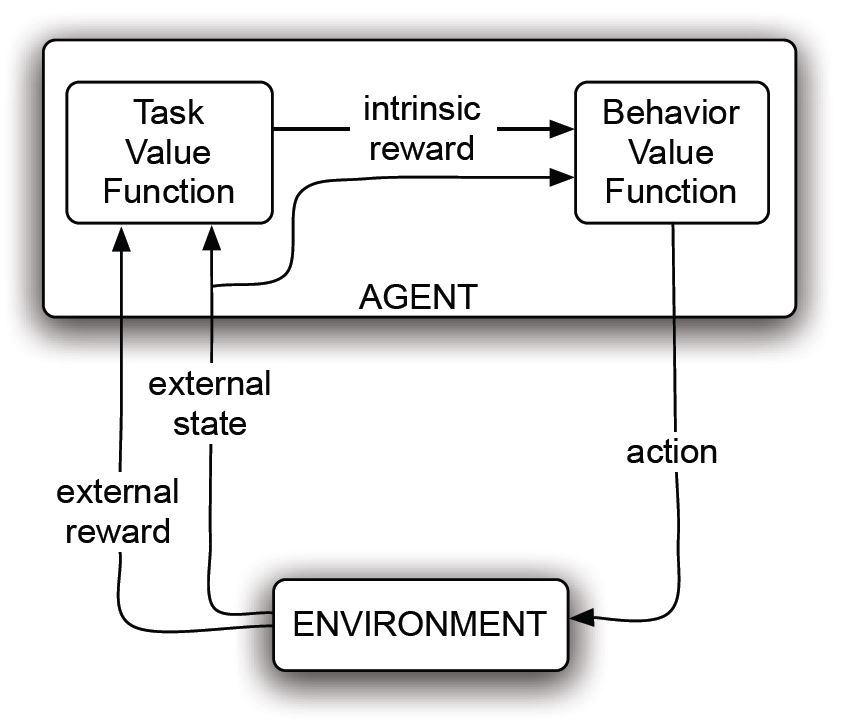
\includegraphics[width=0.5\textwidth]{rw_intrinsic_reward.JPG}
    \caption{Schematische Repräsentation des Algorithmus} \label{img:rwIntrinsicReward}
    \source{\cite{r09_csimcsek2006intrinsic}}
\end{figure}
Hier wird also neben der externen Belohnung eine hiervon abhängige weitere Belohnung erzeugt, welche Auswirkungen auf das Lernverhalten des Agenten hat. Es lässt sich argumentieren, dass diese zweite Belohnung Ähnlichkeiten mit unserer modifizierten Belohnung hat.

Das Konzept von intrinsischen Rewards ist natürlich nicht neu. Der bekannte KI-Forscher Jürgen Schmidhuber erklärt in \cite{r01_schmidhuber2009driven}, dass \textit{curiosity} dazu genutzt werden kann, den Agenten zur aktiven Erkundung der Umgebung anzuregen. Der Agent soll hierfür die beobachteten Daten aufgrund von auftretenden Regularitäten zusammenzufassen. Die komprimierte Version der Daten kann als deren vereinfachte Erklärung aufgefasst werden. Daten, welche sich nicht in bisher bekannte Regelmäßigkeiten einordnen lassen, sollen für den Agenten interessanter sein, da diese zum Erlernen einer besseren Komprimierung aller Daten beitragen. Deshalb erhält der Agent zusätzlich einen internen Reward, wenn er lernt die bisher gesammelten Daten mit weniger Bits darzustellen, welcher zusammen mit dem externen Reward maximiert werden soll. Diese Methode soll auch in Umgebungen mit spärlicher Belohnung dazu führen, dass der Agent diese erkundet und lernt wie sie funktioniert. Dieser intrinsische Reward, welchen Schmidhuber als \textit{curiosity reward} bezeichnet, hat also ebenfalls starke Auswirkung auf das Erkundungs- und Lernverhalten, weswegen wir diesen Ansatz hier erwähnen.

Im Gegensatz zu unserer Idee, den Reward in Bezug auf $ \epsilon $ zu modifizieren, existiert außerdem der gegenteilige Ansatz, den Wert von $ \epsilon $ während des Trainings je nach erhaltenem Reward zu kontrollieren. \cite{r13_dos2017adaptive} nennt dies \textit{adaptive $ \epsilon $-greedy} und geht hierbei so vor, dass nach einer gewissen Anzahl von zufällig gewählten Aktionen überprüft wird, ob die durchschnittliche Belohnung größer ist als beim letzten Mal. Falls ja wird $ \epsilon $ entsprechend angepasst, ist sie geringer, so wird $ \epsilon $ aus 0.5 gesetzt. In Abbildung \ref{img:rwAdaptiveEpsilon} ist diesen Algorithmus dargestellt. 
\begin{figure}[h!]
    \centering
    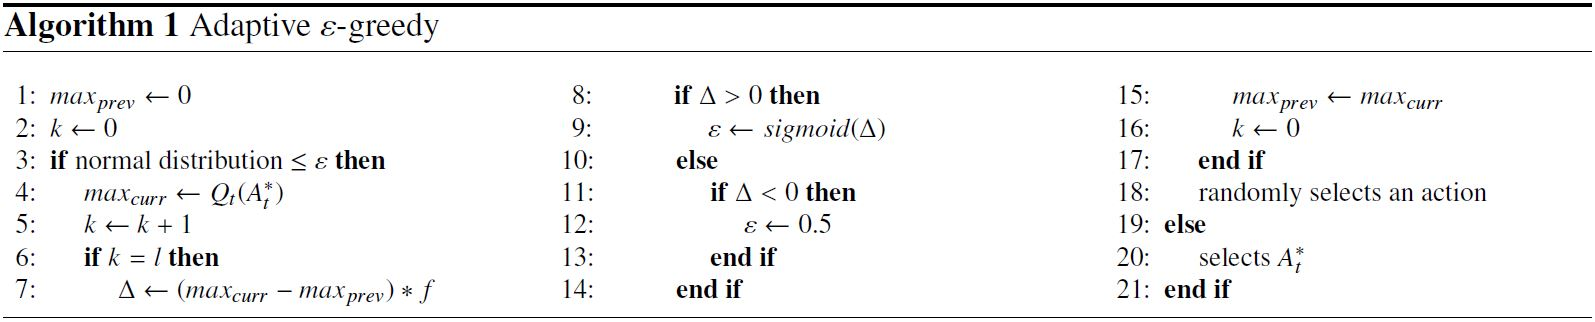
\includegraphics[width=\textwidth]{rw_adaptive_epsilon.JPG}
    \caption{Adaptiver $ \epsilon $-greedy-Algorithmus} \label{img:rwAdaptiveEpsilon}
    \source{\cite{r13_dos2017adaptive}}
\end{figure}
\cite{r13_dos2017adaptive} zeigt, dass die adaptive $ \epsilon $-greedy-Methode in den durchgeführten Experimenten zu besseren Ergebnissen führt als die $ \epsilon $-greedy Methode. Man muss allerdings erwähnen, dass das $ \epsilon $ bei letzterem einen statischen Wert hat.

Eine weitere Lernmethode, die ohne einen Reward auskommt, ist das in \cite{r02_eysenbach2018diversity} beschriebene Erlernen von Fähigkeiten mittels \textit{Diversity}. In einer unüberwachten Phase soll der Agent zunächst eine Menge von Fähigkeiten erlernen, die sich stark voneinander unterscheiden. Hierzu folgt der Agent dem DIAYN-Algorithmus (\glqq Diversity is all you need\grqq{}). Die Belohnung für die einzelnen Aktionen hängt in dieser Phase von der Unterscheidbarkeit der Fähigkeiten ab. Anders gesagt sollen sich die besuchten Zustände so unterschiedlich wie möglich sein.
\begin{figure}[h!]
    \centering
    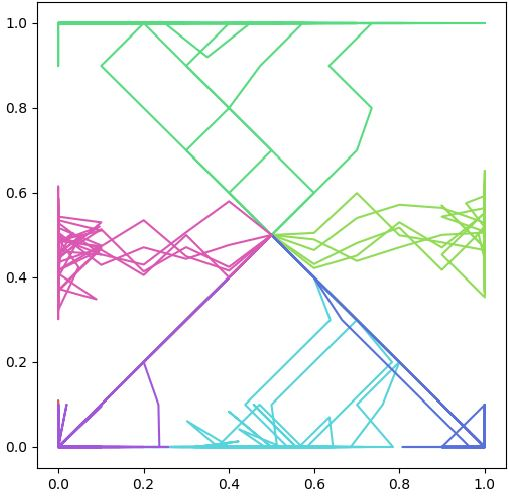
\includegraphics[width=0.4\textwidth]{rw_curiosity.JPG}
    \caption{Mittels DIAYN erlernte Skills in einem 2D-Environment} \label{img:rwCuriosity}
    \source{\cite{r02_eysenbach2018diversity}}
\end{figure}
In Abbildung \ref{img:rwCuriosity} ist das Ergebnis dieser Phase für eine simple 2D Navigation dargestellt. Der Agent startet hier in der Mitte und kann sich im Raum bewegen. Es lässt sich erkennen, dass die erlernten Fähigkeiten, welche hier als farbige Pfade dargestellt sind, aufgrund ihrer Ungleichheit einen Großteil des Zustandsraums abdecken. Wenn nun die Aufgabe in der nächsten Phase lautet, dass der Agent nach unten links gehen soll, so ist der lila Pfad ein sehr vielversprechender Kandidat. Die Tatsache, dass die erlernten Fähigkeiten im Idealfall so unterschiedlich wie möglich sind, stellt nach \cite{r02_eysenbach2018diversity} sicher, dass einige brauchbare Fähigkeiten dabei sind. Soll der Agent nun ein tatsächliches Problem in der Domäne lösen, werden die gefundenen Fähigkeiten als mögliche Aktionen genutzt. \cite{r02_eysenbach2018diversity} zeigt anhand von einigen Experimenten, dass die DIAYN-Methode zu schnelleren Lernerfolgen führt. 


% TODO maybe einleitung? Die Notwendigkeit einer Erkundungsstrategie wird allerdings bereits von \cite{06_sutton2018reinforcement} betont, einem auf dem Gebiet des Reinforcement Learning sehr oft zitiertem Werk. 